\chapter[REFERENCIAL TEÓRICO]{REFERENCIAL TEÓRICO} \label{cap:referencial}

\section{TRABALHOS CORRELATOS}

A base de dados publica 3w foi elaborada por \cite{vargas2019base}, será utilizada como base para aplicação dos algoritmos de redução dimensionalidade não lineares, conforme foi sugerido como trabalhos futuros por \cite{vargas2019base} na sua tese. O autor ainda elaborou um
\textit{benchmark} para detecção de anomalias usando as técnicas de Floresta de Isolamento e OCSVM.

No trabalho de \cite{fernandes2022comparaccao} foi  utilizado o \textit{benchmark} para detecção de anomalias proposto por \cite{vargas2019base}, estendeu seus resultados pois usou mais classificadores (LOF, Envelope Elíptico, Floresta de Isolamento, OCSVM e Redes Neurais do tipo \textit{autoencoders}), nesse trabalho não foi utilizada nenhuma técnica de redução de dimensionalidade, e ele será a base de comparação dos resultados obtidos com as técnicas de dimensionalidade propostas nesse trabalho.

No trabalho elaborado por \cite{rodrigo2021}, utilizou a base de dados pública 3w elaborada por \cite{vargas2019base} para detecção de anomalias, nesse trabalho é observado a etapa de redução de dimensionalidade utilizado a técnica de \textit{autoencoders}, onde os resultados obtidos foram de dezoito pontos percentuais para os modelos OCSVM e dez pontos percentuais para os modelos de Floresta de Isolamento \cite{rodrigo2021},  em comparação com o \textit{benchmark} proposto por\cite{vargas2019base}.



%%% INICIO PARTE REVISÃO
\todo[inline]{INICIO -  APENAS TEXTO BASE }

\section{REDUÇÃO DE DIMENSIONALIDADE}

Após a extração de características, é possível que se tenha uma grande quantidade de características, e pode ser necessário reduzir os custos de processamento. Esse processo é denominado de redução de dimensionalidade. Esta etapa não existiu na abordagem proposta
deste trabalho.
As técnicas mais comuns de redução de dimensionalidade são PCA (Principal Componet Analysis), LDA (Linear Discriminant Analysis) e NMF (Non-negative matrix factorization) (KOWSARI et al., 2019). O Self-Organizing Map (SOM) é um tipo específico de rede neural,
proposto por Kohonen (2013), que também é utilizado como uma ferramenta de redução de
dimensionalidade para extração de características em classificação de dados de alta
dimensionalidade, sendo considerado como uma alternativa ao PCA na detecção e diagnóstico
de falhas para processos industriais complexos (YU et al., 2014).

\subsection{TÉCNICAS DE REDUÇÃO DE DIMENSIONALIDADE NÃO LINEARES}

\subsubsection{KERNEL PRINCIPAL COMPONENT ANALYSIS (KPCA)}
é uma técnica de redução de dimensão não linear (NLDRT) que foi introduzida por. É uma extensão do PCA tradicional que funciona com espaço de recursos de alta dimensão (HD) empregando o método kernel. A diferença entre KPCA e PCA é que existe um cálculo de vetor próprio da matriz kernel com KPCA enquanto o PCA calcula a matriz de covariância [195]. Além disso, componentes principais não lineares podem ser extraídos com menos poder computacional com KPCA. Para dados com variedades não lineares, KPCA oferece boa codificação [196]. Com KPCA, há uma transformação não linear dos dados de entrada do espaço de entrada original para o kernel para cada dado. Uma matriz kernel K é então formada a partir do produto interno do novo recurso. A PCA é consequentemente aplicado o K centralizado na estimação da matriz de covariância dos novos vetores de características [197]. Alguns kernels extensivamente usados incluem Gaussiano, Polinomial e Tangente Hiperbólico e Radial. Uma desvantagem do KPCA é que o custo de computação pode ser extremamente alto, o que pode levar a problemas numéricos de diagonalização de grandes matrizes [197]. Para superar essas desvantagens, Rosipal e Girolami propuseram um algoritmo EM para KPCA [197], que é uma abordagem de maximização de expectativas para realizar análise de componentes principais do kernel e resultados experimentais mostraram que é um método computacionalmente eficiente, especialmente para um grande número de pontos de dados. Uma desvantagem dessa abordagem, no entanto, é que ela ainda precisa armazenar a matriz do kernel N × N, o que limita sua aplicabilidade em muitos problemas de grandes conjuntos de dados. O Block Adaptive KPCA (BAKPCA) foi desenvolvido por  para adicionar novos blocos de forma não iterativa e dinâmica e remover blocos de dados antigos. É eficiente no processamento de sinais e também no monitoramento de processos. O Greedy KPCA também foi proposto por [199] para melhorar o desempenho do classificador SVM. Os resultados mostraram que o kernel ganancioso PCA pode reduzir significativamente a complexidade enquanto mantém a precisão da classificação. No entanto, o Greedy KPCA foi considerado inadequado para remoção de ruído. O Subconjunto KPCA (SKPCA) também foi introduzido por [200] para reduzir complexidades nos cálculos de KPCA para redução de dimensão, bem como classificação. O Robust KPCA também foi proposto por [201] para lidar com outliers e melhorar a precisão da classificação de proteínas. [202] introduziram o PCA discriminativo (dPCA) para análise discriminativa de múltiplos S. Nanga et al. DOI: 10.4236/jdaip.2021.93013 201 Journal of Data Analysis and Information Processing datasets e tem sido aplicado em áreas como dados de saúde, dados de sensores e imagens faciais. A construção supervisionada do kernel para PCA não supervisionado no reconhecimento facial também foi proposta. Os resultados experimentais revelaram que a construção do kernel supervisionado para PCA não supervisionado (SK-PCA) teve um desempenho melhor do que o KPCA com kernel RBF (RBF-PCA) usando bancos de dados ORL e FERET. Os tipos de dados citados na literatura nos quais o KPCA foi aplicado e teve um bom desempenho são Imagem, Áudio , Vídeo e dados de séries temporais.

\subsubsection{ISOMETRIC MAPPING (ISOMAP)}

Outro NLDRT não supervisionado popular cujo objetivo é encontrar intrinsecamente estruturas de dados de uma variedade não linear é o ISOMAP. O algoritmo proposto por [227] tenta extrair parametrizações para conjuntos de dados em um espaço de baixa dimensão para formar um espaço de alta dimensão tal que haja uma preservação das distâncias geodésicas pareadas de modo que pontos próximos estejam distantes no mapa de espaço de alta dimensão para pontos próximos que estão distantes no espaço de baixa dimensão. A característica distintiva do ISOMAP é sua capacidade de obter uma representação dimensional menor dos dados, enquanto a distância geodésica é preservada [227]; [228]. O ISOMAP combina as principais características do PCA e do MDS em termos de eficiência computacional, garantias de convergência assintótica e otimização global com a flexibilidade de uma extensa classe de manifolds não lineares. A abordagem ISOMAP baseia-se basicamente no MDS tradicional, mas a propriedade distintiva é que procura preservar a geometria intrínseca dos dados que são capturados na distância geodésica entre os pares de pontos de dados [227]. O ISOMAP tem sido eficiente quando usado na detecção de irregularidades de análises de vídeo em tempo real [229]. Um ISOMAP baseado em caminho foi proposto por [230] para melhorar a memória e também as complexidades de tempo. O caminho geodésico é usado nesta abordagem para encontrar a incorporação de baixa dimensão. Algumas das desvantagens do ISOMAP são que ele é computacionalmente caro e tem um desempenho ruim quando o manifold não é bem amostrado e contém furos [230]. O Landmark Isomap (L-Isomap) foi apresentado por [231] para melhorar a escalabilidade do Isomap. O ISOMAP foi aplicado com sucesso na condição do tráfego rodoviário urbano [232], sumarização de fala e identificação de rachaduras em materiais [233], reconhecimento facial [234]. Versões supervisionadas do Isomap foram propostas. Isso inclui Isomap Supervisionado para classificação, Isomap Supervisionado com medidas de dissimilaridade na aprendizagem incorporada e Isomap Supervisionado para classificação de imagem de folha de planta [237].

Fig. \ref{fig:ISOMAP} Diagrama esquemático do algoritmo ISOMAP.
  Nota: A: Distância Euclidiana e Distância Geodésica;
  B: diagramas de pontos adjacentes;
C: reduzido a dados bidimensionais.
Uma distância euclidiana (comprimento da linha tracejada) do espaço de entrada de alta dimensão e distância geodésica da variedade de baixa dimensão (comprimento da curva sólida);
B o verdadeiro caminho geodésico no mapa geodésico que é efetivamente calculado através do gráfico de vizinhança G e este caminho é tomado como o caminho mais curto.
  C a incorporação bidimensional recuperada pelo ISOMAP, onde as linhas azuis na

\begin{figure}[H]
    \centering
    \caption{Diagrama esquemático do algoritmo ISOMAP.}. 
    \label{fig:ISOMAP}
 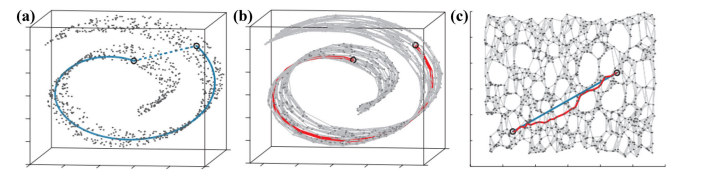
\includegraphics[width=120mm]{images/fig8.png}
    \fonte{\cite{jia2022iso}}
\end{figure}


\subsubsection{DEEP MANIFOLD TRANSFORMATION(DMT)}

é uma rede neural profunda de feed-forward regularizada por restrições de camada cruzada. Uma instância da arquitetura DMT é ilustrada na Fig.1 usando um DMT-AutoEncoder. De um modo geral, uma rede não linear de várias camadas pode suportar um grau mais alto de não linearidade do que redes não lineares de camada única ou equivalentes como t-SNE ou UMAP. O NLDR é realizado usando o DMT-Encoder, que transforma a entrada X em uma incorporação (no espaço latente) Z = X(L) na camada L (a camada latente). Os recursos latentes Z podem ser usados para tarefas posteriores, como visualização e classificação. O DMT-Decoder, que pode assumir uma forma simétrica ao DMT-Encoder, é treinado com as restrições de reconstrução (linhas tracejadas laranja) para reconstruir Z em Xˆ. O codificador DMT aprendido pode ser aplicado.

Figura \ref{fig:li2020DTM}: Ilustração da estrutura de transformação profunda do manifold (DMT) usando um DMT-AutoEncoder (melhor visualizado em cores). Consiste em uma cascata de transformações  (l) (ou ˆ(l) , setas azuis) com as restrições de preservação de geometria local (LGP) entre camadas (mostradas em arcos laranja) impostas entre a camada 0 e a camada L com peso . A restrição de perda de reconstrução com peso  é mostrada em linha tracejada laranja.

\begin{figure}[H]
    \centering
    \caption{Deep manifold transformation (DMT).}. 
    \label{fig:li2020DTM}
 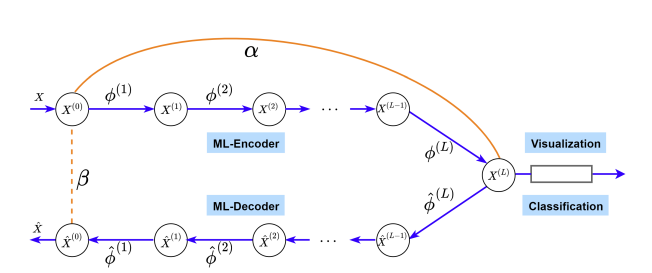
\includegraphics[width=150mm]{images/fig7.png}
    \fonte{\cite{li2020DTM}}
\end{figure}





